\part{Programming Techniques}\label{programming-techniques.part}


\chapter{Print Statements and Debugging}

\noindent
Before getting into specific statistical programming techniques
in the following chapters, this chapter is dedicated to comments
and print statements.

\section{Comments}

Stan supports \Cpp-style comments; see \refsection{comments} for full
details.  The recommended style is to use line-based comments for
short comments on the code or to comment out one or more
lines of code.  Bracketed comments are then reserved for long
documentation comments.  The reason for this convention is that
bracketed comments cannot be wrapped inside of bracketed comments.

\subsection{What Not to Comment}

When commenting code, it is usually safe to assume that you are 
writing the comments for other programmers who understand the basics 
of the programming language in use.  In other words, don't comment the
obvious.  For instance, there is no need to have comments
such as the following, which add nothing to the code.
%
\begin{quote}
\begin{Verbatim}
y ~ normal(0,1);  // y has a unit normal distribution
\end{Verbatim}
\end{quote}
%
A Jacobian adjustment for a hand-coded transform might be worth
commenting, as in the following example.
%
\begin{quote}
\begin{Verbatim}
exp(y) ~ normal(0,1);
lp__ <- lp__ + y;  // log Jacobian of exp(y) inverse transform
\end{Verbatim}
\end{quote}
%
It's an art form to empathize with a future code reader and decide
what they will or won't know (or remember) about statistics and Stan.

\subsection{What to Comment}

It can help to document variable declarations if variables are given
generic names like \code{N}, \code{mu}, and \code{sigma}.  For
example, some data variable declarations in an item-response model
might be usefully commented as follows.
%
\begin{quote}
\begin{Verbatim}
int<lower=1> N;   // number of observations
int<lower=1> I;   // number of students
int<lower=1> J;   // number of test questions
\end{Verbatim}
\end{quote}
%
The alternative is to use longer names that do not require comments.
%
\begin{quote}
\begin{Verbatim}
int<lower=1> n_obs;
int<lower=1> n_students;
int<lower=1> n_questions;
\end{Verbatim}
\end{quote}
%
Both styles reasonable and which one to adopt is mostly a matter of
taste (mostly because sometimes models come with their own naming
conventions which should be followed so as not to confuse readers of
the code familiar with the statistical conventions).

Some code authors like big blocks of comments at the top explaining
the purpose of the model, who wrote it, copyright and licensing
information, and so on.  The following bracketed comment is an
example of a conventional style for large comment blocks.
%
\begin{quote}
\begin{Verbatim}
/*
 * Item-Response Theory PL3 Model
 * -----------------------------------------------------
 * Copyright: Joe Schmoe  <joe@schmoe.com>
 * Date:  19 September 2012
 * License: GPLv3
 */

data {
  ...
\end{Verbatim}
\end{quote}
%
The use of leading asterisks helps readers understand the scope of the
comment.  The problem with including dates or other volatile
information in comments is that they can easily get out of synch with
the reality of the code.  A misleading comment or one that is wrong is
worse than no comment at all!

\section{Print Statements}

Stan supports print statements with one or more string or expression
arguments.  Because Stan is an imperative language, variables can have
different values at different points in the execution of a program.
Print statements can be invaluable for debugging, especially for a
language like Stan with no stepwise debugger.

For instance, to print the value of the expression \code{y} along with
the log probability accumulator, use the following statement.
%
\begin{quote}
\begin{Verbatim}
print("y=", y, " log probability=", lp__);
\end{Verbatim}
\end{quote}
%
This print statement prints the string ``y='' followed by the value of
the expression \code{y}, followed by the string `` log probability=''
(with the leading space), followed by the value of the variable
\Verb|lp__|. 

Each print statement is followed by a new line.  The specific ASCII
character(s) generated to create a new line are platform specific.

Arbitrary expressions can be used.  For example, the statement
\begin{quote}
\begin{Verbatim}
print("1+1=", 1+1);
\end{Verbatim}
\end{quote}
%
will print ``1 + 1 = 2'' followed by a new line.

Print statements may be used anywhere other statements may be used,
but their behavior in terms of frequency depends on how often the
block they are in is evaluated.  See \refsection{print-statements} for
more information on the syntax and evaluation of print statements.


\chapter{Missing Data \& Partially Known Parameters}

\noindent
\BUGS and \R support mixed arrays of known and missing data.  In
\BUGS, known and unknown values may be mixed as long as every unknown
variable appears on the left-hand side of either an assignment or
sampling statement.  

\section{Missing Data}


\Stan treats variables declared in the \code{data} and
\code{transformed data} blocks as known and the variables in the
\code{parameters} block as unknown.

The next section shows how to create a mixed array of known and
unknown values as in \BUGS.  The recommended approach to missing data
in \Stan is slightly different than in \BUGS.  An example involving
missing normal observations%
%
\footnote{A more meaningful estimation example would involve a
  regression of the observed and missing observations using predictors
  that were known for each and specified in the \code{data} block.}
%
could be coded as follows.
%
\begin{quote}
\begin{Verbatim}
data {
  int<lower=0> N_obs;
  int<lower=0> N_miss;
  real y_obs[N_obs];
}
parameters {
  real mu;
  real<lower=0> sigma;
  real y_miss[N_miss];
}
model {
  for (n in 1:N_obs)
    y_obs[n] ~ normal(mu,sigma);
  for (n in 1:N_miss)
    y_miss[n] ~ normal(mu,sigma);
}
\end{Verbatim}
\end{quote}
%
The number of observed and missing data points are coded as data with
non-negative integer variables \code{N\_obs} and \code{N\_miss}.  The
observed data is provided as an array data variable \code{y\_obs}.
The missing data is coded as an array parameter, \code{y\_miss}.  The
ordinary parameters being estimated, the location \code{mu} and scale
\code{sigma}, are also coded as parameters.

The model contains one loop over the observed data and one over the
missing data.  This slight redundancy in specification leads to much
more efficient sampling for missing data problems in \Stan than the
more general technique described in the next section.


\section{Partially Known Parameters}\label{partially-known-parameters.section}

In some situations, such as when a multivariate probability function
has partially observed outcomes or parameters, it will be necessary to
create a vector mixing known (data) and unknown (parameter) values.
This can be done in \Stan by creating a vector or array in the
\code{transformed parameter} block and assigning to it.

The following example involves a bivariate covariance matrix in which the
variances are known, but the covariance is not.
%
\begin{quote}
\begin{Verbatim}
data {
  int<lower=0> N;
  vector[2] y[N];
  real<lower=0> var1;     real<lower=0> var2;
}
transformed data {
  real<lower=0> max_cov;  real<lower=0> min_cov;   
  max_cov <- sqrt(var1 * var2);  
  min_cov <- -max_cov;
}
parameters {
  vector[2] mu;
  real<lower=min_cov,upper=max_cov> cov;
}
transformed parameters {
  matrix[2,2] sigma;
  sigma[1,1] <- var1;     sigma[1,2] <- cov;
  sigma[2,1] <- cov;      sigma[2,2] <- var2;
}  
model {
 for (n in 1:N)
   y[n] ~ multi_normal(mu,sigma);
}
\end{Verbatim}
\end{quote}
%
The variances are defined as data in variables \code{var1} and
\code{var2}, whereas the covariance is defined as a parameter in
variable \code{cov}.  The $2 \times 2$ covariance matrix
\code{sigma} is defined as a transformed parameter, with the variances
assigned to the two diagonal elements and the covariance to the two
off-diagonal elements.

The constraint on the covariance declaration ensures that the
resulting covariance matrix \code{sigma} is positive definite.  The
bound, plus or minus the square root of the product of the variances,
is defined as transformed data so that it is only calculated once.

\section{Efficiency Note}

The missing-data example in the first section could be programmed with
a mixed data and parameter array following the approach of the
partially known parameter example in the second section.  The behavior
will be correct, but the computation is wasteful.  Each parameter, be
it declared in the \code{parameters} or \code{transformed parameters}
block, uses an algorithmic differentiation variable which is more
expensive in terms of memory and gradient-calculation time than a
simple data variable.  Furthermore, the copy takes up extra space and
extra time.


\chapter{Truncated or Censored Data}

\noindent
Data in which measurements have been truncated or censored can be
coded in \Stan following their respective probability models.

\section{Truncated Data}

Truncated data is data for which measurements are only reported if
they fall above a lower bound, below an upper bound, or between a
lower and upper bound.  

Truncated data may be modeled in \Stan using truncated distributions.
For example, suppose the truncated data is $y_n$ with an upper
truncation point of $U = 300$ so that $y_n < 300$.  In \Stan, this
data can be modeled as following a truncated normal distribution for
the observations as follows. 
%
\begin{quote}
\begin{Verbatim} 
data {
   int<lower=0> N;
   real U;
   real<upper=U> y[N];
} 
parameters {
   real mu;
   real<lower=0> sigma;
} 
model {
  for (n in 1:N)
       y[n] ~ normal(mu,sigma) T[,U];
}
\end{Verbatim}
\end{quote}
% 
The model declares an upper bound \code{U} as data and constrains
the data for \code{y} to respect the constraint;  this will be checked
when the data is loaded into the model before sampling begins.

This model implicitly uses an improper flat prior on the scale and
location parameters; these could be given priors in the model using
sampling statements.

\subsection{Constraints and Out-of-Bounds Returns}\label{truncation-constraints.section}

If the sampled variate in a truncated distribution lies outside of
the truncation range, the probability is zero, so the log probability
will evaluate to $-\infty$.  For instance, if variate \code{y} is
sampled with the statement.
%
\begin{quote}
\begin{Verbatim}
for (n in 1:N) 
    y[n] ~ normal(mu,sigma) T[L,U];
\end{Verbatim}
\end{quote}
%
then if the value of \code{y[n]} is less than the value of \code{L}
or greater than the value of \code{U}, the sampling statement produces
a zero-probability estimate.

To avoid variables straying outside of truncation bounds, appropriate
constraints are required.  For example, if \code{y} is a parameter in
the above model, the declaration should constrain it to fall between
the values of \code{L} and \code{U}.
%
\begin{quote}
\begin{Verbatim}
parameters {
    real<lower=L,upper=U> y[N];
    ...
\end{Verbatim}
\end{quote}

If in the above model, \code{L} or \code{U} is a parameter and
\code{y} is data, then \code{L} and \code{U} must be appropriately
constrained so that all data is in range and the value of \code{L} is
less than that of \code{U} (if they are equal, the parameter range
collapses to a single point and the Hamiltonian dynamics used by 
the sampler break down).  The following declarations ensure the bounds
are well behaved.
%
\begin{quote}
\begin{Verbatim}
parameters {
    real<upper=min(y)> L; // L < y[n]
    real<lower=fmax(L,max(y))> U; // L < U; y[n] < U
\end{Verbatim}
\end{quote}
%
Note that for pairs of real numbers, the function \code{fmax} is used
rather than \code{max}.







\subsection{Unknown Truncation Points}

If the truncation points are unknown, they may be estimated as
parameters.  This can be done with a slight rearrangement of the
variable declarations from the model in the previous section with
known truncation points.
%
\begin{quote}
\begin{Verbatim}
data {
   int<lower=1> N;
   real y[N];
}
parameters
   real<upper = min(y)> L; 
   real<lower = max(y)> U;
   real mu;
   real<lower=0> sigma;
}
model {
  L ~ ...;  
  U ~ ...;
  for (n in 1:N)
       y[n] ~ normal(mu,sigma) T[L,U];
}
\end{Verbatim}
\end{quote}
%
Here there is a lower truncation point \code{L} which is declared to
be less than or equal to the minimum value of \code{y}.  The upper
truncation point \code{U} is declared to be larger than the maximum
value of \code{y}.  This declaration, although dependent on the data,
only enforces the constraint that the data fall within the truncation
bounds.  With \code{N} declared as type \code{int<lower=1>}, there must be
at least one data point.  The constraint that \code{L} is less than
\code{U} is enforced indirectly, based on the non-empty data.

The ellipses where the priors for the bounds \code{L} and \code{U}
should go should be filled in with a an informative prior in
order for this model to not concentrate \code{L} strongly around 
\code{min(y)} and \code{U} strongly around \code{max(y)}.


\section{Censored Data}

Censoring hides values from points that are too large, too small, or
both.  Unlike with truncated data, the number of data points that were
censored is known.  The textbook example is the household scale which
does not report values above 300 pounds.  

\subsection{Estimating Censored Values}

One way to model censored data is to treat the censored data as
missing data that is constrained to fall in the censored range of
values.  Because \Stan does not allow unknown values in its arrays or
matrices, the censored values must be represented explicitly.
%
\begin{quote}
\begin{Verbatim}
data {
   int<lower=0> N_obs;
   int<lower=0> N_cens;
   real<lower=0> y_obs[N_obs];
   real<lower=max(y_obs)> U;
}
parameters {
  real<lower=U> y_cens[N_cens];
  real mu;
  real<lower=0> sigma;
}
model {
   for (n in 1:N_obs)
       y_obs[n] ~ normal(mu,sigma);
   for (n in 1:N_cens)
       y_cens[n] ~ normal(mu,sigma);
}
\end{Verbatim}
\end{quote}
%
Because the censored data array \code{y\_cens} is declared to be a parameter, it
will be sampled along with the location and scale parameters \code{mu}
and \code{sigma}.  Because the censored data array \code{y\_cens} is
declared to have values of type \code{real<lower=U>}, all imputed values
for censored data will be greater than \code{U}.  The imputed censored
data affects the location and scale parameters through the last
sampling statement in the model.  

\subsection{Integrating out Censored Values}

Although it is wrong to ignore the censored values in estimating
location and scale, it is not necessary to impute values.  Instead,
the values can be integrated out.  Each censored data point has a
probability of
%
\[
\mbox{Pr}[y > U] 
= \int_U^{\infty} \distro{Normal}(y|\mu,\sigma) \, dy
= 1 - \Phi\left(\frac{y - \mu}{\sigma}\right),
\]
%
where $\Phi()$ is the unit normal cumulative distribution function.
With $M$ censored observations, the total probability on the log scale
is
\[
\log \prod_{m=1}^M \mbox{Pr}[y_m > U]
= \log \left( 1 - \Phi\left(\frac{y - \mu}{\sigma}\right)\right)^{M}
= M \, \log \left( 1 - \Phi\left(\frac{y - \mu}{\sigma}\right)\right)
\]
% 
Although \Stan implements $\Phi$ with the function $\code{Phi}$, \Stan
also provides the cumulative distribution function \code{normal\_cdf},
defined by
\[
\code{normal\_cdf}(y,\mu,\sigma) = \Phi \left( \frac{y - \mu}{\sigma} \right).
\]
%
The following model assumes
that the censoring point is known, so it is declared as data.
%
\begin{quote}
\begin{Verbatim}
data {
   int<lower=0> N_obs;
   int<lower=0> N_cens;
   real<lower=0> y_obs[N_obs];
   real<lower=max(y_obs)> U;
}
parameters {
  real mu;
  real<lower=0> sigma;
}
model {
   for (n in 1:N_obs)
       y_obs[n] ~ normal(mu,sigma); 
   lp__ <- lp__ + N_cens * log1m(normal_cdf(U,mu,sigma));
}
\end{Verbatim}
\end{quote}
%
For the observed values in \Verb|y_obs|, the normal sampling model is
used without truncation.  The log probability accumulator
\Verb|lp__| is directly incremented using the calculated log
cumulative normal probability of the censored data items.  The
built-in function \code{log1m} is used, which maps $x$ to $\log (1 -
x)$ in an arithmetically stable way for values of $x$ near zero.

To deal with situations where the censoring point variable \code{U} is
unknown, the declaration of \code{U} should be moved from the data
block to the parameters block.



\chapter{Mixture Modeling}\label{mixture-modeling.chapter}

\noindent
Mixture models of an outcome assume that the outcome is drawn from one
of several distributions, the identity of which is controlled by a
categorical mixing distribution. Mixture models typically have
multimodal densities with modes near the modes of the mixture
components.  Mixture models may be parameterized in several ways,
as described in the following sections.


\section{Latent Discrete Parameterization}

One way to parameterize a mixture model is with a latent categorical
variable indicating which mixture component was responsible for the
outcome. For example, consider $K$ normal distributions with locations
$\mu_k \in \reals$ and scales $\sigma_k \in (0,\infty)$.  Now consider
mixing them in proportion $\theta$, where $\theta_k \geq 0$ and
$\sum_{k=1}^K \theta_k = 1$ (i.e., $\theta$ lies in the unit $K$-simplex).
For each outcome $y_n$ there is a latent variable $z_n$ in
$\setlist{1,\ldots,K}$ with a categorical distribution parameterized
by $\theta$,
%
\[
z_n \sim \distro{Categorical}(\theta).
\]
%
The variable $y_n$ is distributed according to the parameters
of the mixture component $z_n$, 
\[
y_n \sim \distro{Normal}(\mu_{z[n]},\sigma_{z[n]}).
\]
%
This model is not directly supported by \Stan because it involves
discrete parameters $z_n$, but \Stan can sample $\mu$ and $\sigma$ 
by summing out the $z$ parameter as described in the next section.


\section{Summing out the Responsibility Parameter}

To implement the normal mixture model outlined in the previous
section in \Stan, the discrete parameters can be summed out of the
model. If $Y$ is a mixture of $K$ normal distributions with 
locations $\mu_k$ and scales $\sigma_k$ with mixing proportions
$\theta$ in the unit $K$-simplex, then 
\[
p_Y(y) = \sum_{k=1}^K \theta_k \, \distro{Normal}(\mu_k,\sigma_k).
\]

For example, the mixture of $\code{Normal}(-1,2)$ and
$\code{Normal}(3,1)$ with mixing proportion $\theta =
(0.3,0.7)^{\top}$ can be implemented in \Stan as follows.
%
\begin{quote}
\begin{Verbatim}
parameters {
  real y;
}
model {
   lp__ <- log_sum_exp(log(0.3) + normal_log(y,-1,2),
                       log(0.7) + normal_log(y,3,1));
}
\end{Verbatim}
\end{quote}
%
The log probability term is derived by taking
\begin{eqnarray*}
\log p_Y(y) & = & \log \, \left( 0.3 \times \distro{Normal}(y|-1,2) \, + \,
  0.7 \times
  \distro{Normal}(y|3,1) \, \right)
\\[2pt]
& = & \log(\! \begin{array}[t]{l}
                 \exp(\log(0.3 \times \distro{Normal}(y|-1,2))) \\
                 + \exp(\log(0.7 \times \distro{Normal}(y|3,1))) \ )
              \end{array}
% \\[4pt]
% & = & \log( \! \begin{array}[t]{l}\exp(\log(0.3) + \log \distro{Normal}(y|-1,2))
%             \\
%            + \exp(\log(0.7) + \log \distro{Normal}(y|3,1)) \ )
%             \end{array}
\\[2pt]
& = & \mbox{log\_sum\_exp}(\! \begin{array}[t]{l}
                         \log(0.3) + \log \distro{Normal}(y|-1,2),
                         \\                  
                         \log(0.7) + \log \distro{Normal}(y|3,1) \ ).
                       \end{array}
\end{eqnarray*}

Given the scheme for representing mixtures, it may be moved to an
estimation setting, where the locations, scales, and mixture
components are unknown.  Further generalizing to a number of mixture
components specified as data yields the following model.
%
\begin{quote}
\begin{Verbatim}
data {
  int<lower=1> K;          // number of mixture components
  int<lower=1> N;          // number of data points
  real y[N];               // observations
}
parameters {
  simplex[K] theta;        // mixing proportions
  real mu[K];              // locations of mixture components
  real<lower=0> sigma[K];  // scales of mixture components
}
model {
  real ps[K];              // temp for log component densities
  for (k in 1:K) {
    mu[k] ~ normal(0,10);
    sigma[k] ~ uniform(0,10);
  }
  for (n in 1:N) {
    for (k in 1:K) {
      ps[k] <- log(theta[k]) 
               + normal_log(y[n],mu[k],sigma[k]);
    }
    lp__ <- lp__ + log_sum_exp(ps);    
  }
}
\end{Verbatim}
\end{quote}
%
The model involves \code{K} mixture components and \code{N} data
points.  The mixing proportion parameter \code{theta} is declared to
be a unit $K$-simplex, whereas the component location parameter
\code{mu} and scale parameter \code{sigma} are both defined to be
arrays of size \code{K}.  The values in the scale array \code{sigma}
are constrained to be non-negative.  The model declares a local 
array variable \code{ps} to be size \code{K} and uses it to
accumulate the contributions from the mixture components.

The locations and scales are drawn from simple priors for the sake of
this example, but could be anything supported by \Stan.  The mixture
components  could even be modeled hierarchically.

The main action is in the loop over data points \code{n}.  For each
such point, the log of $\theta_k \times
\distro{Normal}(y_n|\mu_k,\sigma_k)$ is calculated and added to the
array \code{ps}.  Then the log probability is incremented with the log
sum of exponentials of those values.





\chapter{Regression Models}

\noindent
\Stan supports regression models from simple linear regressions to
multilevel generalized linear models.  Coding regression models in
\Stan is very much like coding them in \BUGS.

\section{Linear Regression}

The simplest linear regression model is the following, with a single
predictor and a slope and intercept coefficient, and normally
distributed noise.  This model can be written using standard
regression notation as
%
\[
Y_n = \alpha + \beta x_n + \epsilon_n
\ \ \ \mbox{where} \ \ \ 
\epsilon_n \sim \distro{Normal}(0,\sigma).
\]
This is equivalent to the following sampling involving the
residual,
\[
Y_n - (\alpha + \beta X_n) \sim \distro{Normal}(0,\sigma),
\]
and reducing still further, to
\[
Y_n \sim \distro{Normal}(\alpha + \beta X_n, \, \sigma).
\]
%
This latter form of the model is coded in \Stan as follows.
%
\begin{quote}
\begin{Verbatim}
data {
   int<lower=0> N;
   real x[N];
   real y[N];
}
parameters {
    real alpha;
    real beta;
    real<lower=0> sigma;
}
model {
    for (n in 1:N)
        y[n] ~ normal(alpha + beta * x[n], sigma);
}
\end{Verbatim}
\end{quote}
%
There are \code{N} observations, each with predictor \code{x[n]} and
outcome \code{y[n]}.  The intercept and slope parameters are
\code{alpha} and \code{beta}.  The model assumes a normally
distributed noise term with scale \code{sigma}.  This model has
improper priors for the two regression coefficients.

\section{Coefficient and Noise Priors}

There are several ways in which this model can be generalized.  
For example, weak priors can be assigned to the coefficients as follows.
%
\begin{quote}
\begin{Verbatim}
    alpha ~ normal(0,100);
    beta ~ normal(0,100);
    sigma ~ uniform(0,100);
\end{Verbatim}
\end{quote}
%
More informative priors based the (half) Cauchy distribution are coded
as follows.
%
\begin{quote}
\begin{Verbatim}
    alpha ~ cauchy(0,2.5);
    beta ~ cauchy(0,2.5);
    sigma ~ cauchy(0,2.5);
\end{Verbatim}
\end{quote}
%
The regression coefficients \code{alpha} and \code{beta} are
unconstrained, but \code{epsilon} must be positive and properly
requires the half-Cauchy distribution, which would be expressed in
\Stan using truncation as follows.
%
\begin{quote}
\begin{Verbatim}
    sigma ~ cauchy(0,2.5) T[0,];
\end{Verbatim}
\end{quote}
%
Because the log probability function need not be normalized, the extra
factor of 2 is not needed in the model, so the simpler un-truncated
distribution suffices.

\section{Robust Noise Models}

The standard approach to linear regression is to model the noise
term $\epsilon$ as having a normal distribution.  From \Stan's
perspective, there is nothing special about normally distributed
noise.  For instance, robust regression can be accommodated by giving
the noise term a Student-$t$ distribution.  To code this in \Stan, the
sampling distribution is changed to the following.
%
\begin{quote}
\begin{Verbatim}
data {
  ...
  real<lower=0> nu;
}
...
model {
  for (n in 1:N)
    y[n] ~ student_t(nu, alpha + beta * x[n], sigma);
}
\end{Verbatim}
\end{quote}
%
The degrees of freedom constant \code{nu} is specified as data.

\section{Logistic and Probit Regression}\label{logistic-probit-regression.section}

For binary outcomes, either of the closely related logistic or probit
regression models may be used.  These generalized linear models vary
only in the link function they use to map linear predictions in
$(-\infty,\infty)$ to probability values in $(0,1)$.  Their respective
link functions, the logistic function and the unit normal cumulative distribution
function, are both sigmoid functions (i.e., they are both {\it S}-shaped).

A logistic regression model with one predictor and an intercept is coded as
follows.
%
\begin{quote}
\begin{Verbatim}
data {
    int<lower=0> N;
    real x[N];
    int<lower=0,upper=1> y[N];
}
parameters {
    real alpha;
    real beta;
}
model {
    for (n in 1:N)
        y[n] ~ bernoulli(inv_logit(alpha + beta * x[n]));
} 
\end{Verbatim}
\end{quote}
%
The noise parameter is built into the Bernoulli formulation here
rather than specified directly.

Logistic regression is a kind of generalized linear model with binary
outcomes and the log odds (logit) link function.  The inverse of the
link function appears in the model.  

Other link functions may be used in the same way.  For example, probit
regression uses the cumulative normal distribution function, which is
typically written as 
\[
\Phi(x) = \int_{-\infty}^x \distro{Normal}(y|0,1) \, dy.
\]
%
The cumulative unit normal distribution function $\Phi$ is implemented
in \Stan as the function \code{Phi}.  The probit regression model
may be coded in \Stan by replacing the logistic model's sampling
statement with the following.
%
\begin{quote}
\begin{Verbatim}
        y[n] ~ bernoulli(Phi(alpha + beta * x[n]));
\end{Verbatim}
\end{quote}

\section{Multi-Logit Regression}

Multiple outcome forms of logistic regression can be coded directly in
\Stan.  For instance, suppose there are $K$ possible outcomes for each
output variable $y_n$.  Also suppose that there is a $D$-dimensional
vector $x_n$ of predictors for $y_n$.  The multi-logit model with
$\distro{Normal}(0,5)$ priors on the coefficients is coded as follows.
%
\begin{quote}
\begin{Verbatim}
data {
   int<lower=2> K;
   int<lower=0> N;
   int<lower=1> D;
   int<lower=1,upper=K> y[N];
   vector[D] x[N];
}
parameters {
   matrix[K,D] beta;
}
model {
  for (k in 1:K)
    for (d in 1:D)
      beta[k,d] ~ normal(0,5);
  for (n in 1:N)
     y[n] ~ categorical(softmax(beta * x[n]));
}
\end{Verbatim}
\end{quote}
%
The softmax function is defined for a $K$-vector $\gamma \in \reals^K$ by
\[
\mbox{softmax}(\gamma) = 
\left(
 \frac{\exp(\gamma_1)}
      {\sum_{k=1}^K \exp(\gamma_k)},
  \ldots,
  \frac{\exp(\gamma_K)}
       {\sum_{k=1}^K \exp(\gamma_k)}
\right).
\]
%
The result is in the unit $K$-simplex and thus appropriate to use as
the parameter for a categorical distribution.

\subsection{Identifiability}

Because softmax is invariant under adding a constant to each component
of its input, the model is typically only identified if there is a
suitable prior on the coefficients.

An alternative is to use $K-1$ vectors by fixing one of them to be
zero.  See \refsection{partially-known-parameters} for an example of
how to mix known quantities and unknown quantities in a vector.


\section{Ordered Logistic and Probit Regression}\label{ordered-logistic.section}

Ordered regression for an outcome $y_n \in \setlist{1,\ldots,K}$ with
predictors $x_n \in \reals^D$ is determined by a single coefficient
vector $\beta \in \reals^D$ along with a sequence of cutpoints $c \in
\reals^{D-1}$ sorted so that $c_d < c_{d+1}$.  The discrete output is
$k$ if the linear predictor $x_n \beta$ falls between $c_{k-1}$ and
$c_k$, assuming $c_0 = -\infty$ and $c_K = \infty$.  The noise term is
fixed by the form of regression, with examples for ordered logistic
and ordered probit models.  

\subsection{Ordered Logistic Regression}

The ordered logistic model can be coded in \Stan using the
\code{ordered} data type for the cutpoints and the built-in
\code{ordered\_logistic} distribution.
%
\begin{quote}
\begin{Verbatim} 
data {
  int<lower=2> K;
  int<lower=0> N;
  int<lower=1> D;
  int<lower=1,upper=K> y[N];
  row_vector[D] x[N];
} 
parameters {
  vector[D] beta;
  ordered[K-1] c;
} 
model {
  for (n in 1:N)
      y[n] ~ ordered_logistic(x[n] * beta, c);
}
\end{Verbatim}
\end{quote}
% 
The vector of cutpoints \code{c} is declared as \code{ordered[K-1]},
which guarantees that \code{c[k]} is less than \code{c[k+1]}. 

If the cutpoints were assigned independent priors, the constraint
effectively truncates the joint prior to support over points that
satisfy the ordering constraint.  Luckily, \Stan does not need to
compute the effect of the constraint on the normalizing term because
the probability is only needed up to a proportion.


\subsubsection{Ordered Probit}

An ordered probit model could be coded in a manner similar to the
\BUGS encoding of an ordered logistic model.
%
\begin{quote}
\begin{Verbatim}
data {
  int<lower=2> K;
  int<lower=0> N;
  int<lower=1> D;
  int<lower=1,upper=K> y[N];
  row_vector[D] x[N];
}
parameters {
  vector[D] beta;
  ordered[K-1] c;
}
model {
  vector[K] theta;
  for (n in 1:N) {
      real eta;
      eta <- x[n] * beta;
      theta[1] <- 1 - Phi(eta - c[1]);
      for (k in 2:(K-1))
          theta[k] <- Phi(eta - c[k-1]) - erf(eta - c[k]);
      theta[K] <- Phi(eta - c[K-1]);
      y[n] ~ categorical(theta);
  }
}
\end{Verbatim}
\end{quote}
%
The logistic model could also be coded this way by replacing
\code{Phi} with \code{inv\_logit}, though the built-in encoding based
on the softmax transform is more efficient and more numerically
stable.  A small efficiency gain could be achieved by computing the
values \code{Phi(eta - c[k])} once and storing them for re-use.

\section{Hierarchical Logistic Regression}

The simplest multilevel model is a hierarchical model in which the
data is grouped into $L$ distinct categories (or levels).  An extreme approach would be to
completely pool all the data and estimate a common vector of
regression coefficients $\beta$.  At the other extreme, an approach
would no pooling assigns each level $l$ its own coefficient vector
$\beta_l$ that is estimated separately from the other levels.  A
hierarchical model is an intermediate solution where the degree of
pooling is determined by the data and a prior on the amount of
pooling.

Suppose each binary outcome $y_n \in \setlist{0,1}$ has an associated
level, $ll_n \in \setlist{1,\ldots,L}$.  Each outcome will also have
an associated predictor vector $x_n \in \reals^D$.  Each level $l$
gets its own coefficient vector $\beta_l \in \reals^D$.  The
hierarchical structure involves drawing the coefficients $\beta_{l,d}
\in \reals$ from a prior that is also estimated with the data.  This
hierarchically estimated prior determines the amount of pooling.  If
the data in each level are very similar, strong pooling will be
reflected in low hierarchical variance.  If the data in the levels are
dissimilar, weaker pooling will be reflected in higher hierarchical variance.

The following model encodes a hierarchical logistic regression model
with a hierarchical prior on the regression coefficients.
%
\begin{quote}
\begin{Verbatim}
data {
    int<lower=1> D;
    int<lower=0> N;
    int<lower=1> L;
    int<lower=0,upper=1> y[N];
    int<lower=1,upper=L> ll[N];
    row_vector[D] x[N];
}
parameters {
    real mu[D];
    real<lower=0> sigma[D];
    vector[D] beta[L];
}
model {
    for (d in 1:D) {
        mu[d] ~ normal(0,100);
        sigma[d] ~ uniform(0,1000);
        for (l in 1:L)
            beta[l,d] ~ normal(mu[d],sigma[d]);
    }
    for (n in 1:N)
        y[n] ~ bernoulli(inv_logit(x[n] * beta[ll[n]]));
}
\end{Verbatim}
\end{quote}   


\section{Item-Response Theory Models}

Item-response theory (IRT) models the situation in which a number of
students each answer one or more of a group of test questions.  The
model is based on parameters for the ability of the students, the
difficulty of the questions, and in more articulated models, the
discimrinativess of the questions and the probability of guessing
correctly; see \citep[pps.~314--320]{GelmanHill:2007} for a textbook
introduction to hierarchical IRT models and \citep{Curtis:2010} for
encodings of a range of IRT models in BUGS.


\subsection{Data Declaration with Missingness}

The data provided for an IRT model may be declared as follows
to account for the fact that not every student is required to answer
every question.
%
\begin{quote}
\begin{Verbatim}
data {
  int<lower=1> J;              // number of students
  int<lower=1> K;              // number of questions
  int<lower=1> N;              // number of observations
  int<lower=1,upper=J> jj[N];  // student for observation n
  int<lower=1,upper=K> kk[N];  // question for observation n
  int<lower=0,upper=1> y[N];   // correctness for observation n
}
\end{Verbatim}
\end{quote}
%
This declares a total of \code{N} student-question pairs in the data
set, where each \code{n} in \code{1:N} indexes a binary observation
\code{y[n]} of the correctness of the answer of student \code{jj[n]}
on question \code{kk[n]}.

The prior hyperparameters will be hard coded in the rest of this
section for simplicity, though they could be coded as data in
Stan for more flexibility.

\subsection{1PL (Rasch) Model}

The 1PL item-response model, also known as the Rasch model, has one
parameter (1P) for questions and uses the logistic link function (L).
This model is distributed with Stan in the file
\url{src/models/misc/irt/irt.stan}.

The model parameters are declared as follows.
%
\begin{quote}
\begin{Verbatim} 
parameters {    
  real delta;         // mean student ability
  real alpha[J];      // ability of student j - mean ability
  real beta[K];       // difficulty of question k
}
\end{Verbatim}
\end{quote}
%
The parameter \code{alpha[j]} is the ability coefficient for student
\code{j} and \code{beta[k]} is the difficulty coefficient for question
\code{k}.  The non-standard parameterization used here also includes
an intercept term \code{delta}, which represents the average student's
response to the average question.%
%
\footnote{\citep{GelmanHill:2007} treat the $\delta$ term equivalently
  as the location parameter in the distribution of student abilities.}
%
The model itself is as follows.
%
\begin{quote}
\begin{Verbatim} 
model {
  alpha ~ normal(0,1);         // informative true prior
  beta ~ normal(0,1);          // informative true prior
  delta ~ normal(.75,1);       // informative true prior
  for (n in 1:N)
    y[n] ~ bernoulli_logit(alpha[jj[n]] - beta[kk[n]] + delta);
}
\end{Verbatim}
\end{quote}
%
This model uses the logit-parameterized Bernoulli distribution, where
\[
\code{bernoulli\_logit}(y|\alpha) =
\code{bernoulli}(y|\mbox{logit}^{-1}(\alpha)).
\]
%
The key to understanding it is the term inside the
\code{bernoulli\_logit} distribution, from which it follows that
\[
\mbox{Pr}[Y_n = 1] = \mbox{logit}^{-1}(\alpha_{jj[n]} - \beta_{kk[n]}
+ \delta).
\]
%
The model suffers from additive identifiability issues without the
priors.  For example, adding a term $\xi$ to each $\alpha_j$ and
$\beta_k$ results in the same predictions.  The use of priors for
$\alpha$ and $\beta$ located at 0 identifies the parameters; see
\citep{GelmanHill:2007} for a discussion of identifiability issues and
alternative approaches to identification.  

For testing purposes, the IRT 1PL model distributed with Stan uses
informative priors that match the actual data generation process used
to simulate the data in R (the simulation code is supplied in the same
directory as the models).  This is unrealistic for most practical
applications, but allows Stan's inferences to be validated.  A simple
sensitivity analysis with fatter priors shows that the posterior is
fairly sensitive to the prior even with 400 students and 100 questions
and only 25\% missingness at random.  For real applications, the
priors should be fit hierarchically along with the other parameters,
as described in the next section.


\subsection{Multilevel 2PL Model}

The simple 1PL model described in the previous section is generalized
in this section with the addition of a discrimination parameter to
model how noisy a question is and by adding multilevel priors for the
student and question parameters.

The model parameters are declared as follows.
%
\begin{quote}
\begin{Verbatim}
parameters {    
  real delta;                  // mean student ability
  real alpha[J];               // ability for j - mean
  real beta[K];                // difficulty for k
  real log_gamma[K];           // discrim for k
  real<lower=0> sigma_alpha;   // sd of abilities
  real<lower=0> sigma_beta;    // sd of difficulties 
  real<lower=0> sigma_gamma;   // sd of log discrim
}
\end{Verbatim}
\end{quote}
%
The parameters should be clearer after the model definition.
%
\begin{quote}
\begin{Verbatim}
model {
  alpha ~ normal(0,sigma_alpha); 
  beta ~ normal(0,sigma_beta);   
  log_gamma ~ normal(0,sigma_gamma);
  delta ~ cauchy(0,5);
  sigma_alpha ~ cauchy(0,5);
  sigma_beta ~ cauchy(0,5);
  sigma_gamma ~ cauchy(0,5);
  for (n in 1:N)
    y[n] ~ bernoulli_logit( 
               exp(log_gamma[kk[n]])
               * (alpha[jj[n]] - beta[kk[n]] + delta) );
}
\end{Verbatim}
\end{quote}
%
First, the predictor inside the \code{bernoulli\_logit} term is
equivalent to the predictor of the 1PL model multipled by the
discriminativeness for the question, \code{exp(log\_gamma[kk[n]])}.
The parameter \code{log\_gamma[k]} represents how discriminative a
question is, with log discriminations above 0 being less (because
their exponentiation drives the predictor away from zero, which drives
the prediction away from 0.5) and discriminations below 0 being more
noisy (driving the predictor toward zero and hence the prediction
toward 0.5).

The intercept term \code{delta} can't be modeled hierarchically, so it
is given a weakly informative $\distro{Cauchy}(0,5)$ prior.
Similarly, the scale terms, \code{sigma\_alpha}, \code{sigma\_beta},
and \code{sigma\_gamma}, are given half-Cauchy priors.  The truncation
in the half-Cauchy prior is implicit; explicit truncation is not
necessary because the log probabilty need only be calculated up to a
proportion and the scale variables are constrained to $(0,\infty)$ by 
their declarations.



\section{Autoregressive Models}

A first-order autoregressive model (AR(1)) with normal noise takes
each point $y_n$ in a sequence $y$ to be generated according to
%
\[
y_n \sim \distro{Normal}(\alpha + \beta y_{n-1}, \sigma).
\]
%
That is, the expected value of $y_n$ is $\alpha + \beta y_{n-1}$, with
noise scaled as $\sigma$.

\subsection{AR(1) Models}

With improper flat priors on the regression coefficients for slope
($\beta$), intercept ($\alpha$), and noise scale ($\sigma$),
the \Stan program for the AR(1) model is as follows.
%
\begin{quote}
\begin{Verbatim}
data {
    int<lower=0> N;
    real y[N];
}
parameters {
    real alpha;
    real beta;
    real sigma;
}
model {
    for (n in 2:N)
       y[n] ~ normal(alpha + beta*y[n-1], sigma);
}
\end{Verbatim}
\end{quote}
%
The first observed data point, \code{y[1]}, is not modeled here.  

\subsection{Extensions to the Model} 

Proper priors of a range of different families may be added for the
regression coefficients and noise scale.  The normal noise model can
be changed to a Student-$t$ distribution or any other distribution
with unbounded support.  The model could also be made hierarchical if
multiple series of observations are available.  

To enforce the estimation of a stationary AR(1) process, the slope
coefficient \code{beta} may be constrained with bounds as follows.
%
\begin{quote}
\begin{Verbatim}
    real<lower=-1,upper=1> beta;
\end{Verbatim}
\end{quote}
%
In practice, such a constraint is not recommended.  If the data is not
stationary, it is best to discover this while fitting the model.
Stationary parameter estimates can be encouraged with a prior favoring
values of \code{beta} near zero.


\subsection{AR(2) Models}

Extending the order of the model is also straightforward.  For
example, an AR(2) model could be coded with the second-order
coefficient \code{gamma} and the following model statement.
%
\begin{quote}
\begin{Verbatim}
for (n in 3:N)
  y[n] ~ normal(alpha + beta*y[n-1] + gamma*y[n-2], sigma);
\end{Verbatim}
\end{quote}


\subsection{AR($K$) Models}

A general model where the order is itself given as data can be coded
by putting the coefficients in an array and computing the linear
predictor in a loop.
%
\begin{quote}
\begin{Verbatim}
data {
    int<lower=0> K;
    int<lower=0> N;
    real y[N];
}
parameters {
    real alpha;
    real beta[K];
    real sigma;
}
model {
    for (n in (K+1):N) {
        real mu;
    mu <- alpha;
    for (k in 1:K)
        mu <- mu + beta[k] * y[n-k];
    y[n] ~ normal(mu, sigma);
  }
}
\end{Verbatim}
\end{quote}

\chapter{Reparameterizations and Changes of Variables}
\label{change-of-variables.chapter}

\noindent
As with BUGS, Stan supports a direct encoding of reparameterizations.
Stan also supports changes of variables by directly incrementing the
log probability accumulator with the log Jacobian of the transform.

\section{Reparameterizations}

Reparameterizations may be implemented straightforwardly.  For
example, the Beta distribution is parameterized by two positive count
parameters $\alpha, \beta > 0$.  The following example illustrates a
hierarchical Stan model with a vector of parameters \code{theta} are
drawn i.i.d.\ fro a Beta distribution whose parameters are themselves
drawn from a hyperprior distribution.
%
\begin{quote}
\begin{Verbatim}
parameters {
  real<lower = 0> alpha;
  real<lower = 0> beta;
  ...
model {
  alpha ~ ...
  beta ~ ...
  for (n in 1:N)
    theta[n] ~ beta(alpha,beta);
  ...
\end{Verbatim}
\end{quote}

It is often more natural to specify hyperpriors in terms of
transformed parameters.  In the case of the Beta, the obvious choice
for reparameterization is in terms of a mean parameter 
\[
\phi = \alpha / (\alpha + \beta)
\]
and total count parameter
\[
\lambda = \alpha + \beta.
\]
Following \citep[Chapter 5]{GelmanCarlinSternRubin:2003}, the mean
gets a uniform prior and the count parameter a Pareto prior with
$p(\lambda) \propto \lambda^{-2.5}$.
%
\begin{quote}
\begin{Verbatim}
parameters {
  real<lower=0,upper=1> phi;
  real<lower=0.1> lambda;
  ...
transformed parameters {
  real<lower=0> alpha;
  real<lower=0> beta;
  ...
  alpha <- lambda * phi;
  beta <- lambda * (1 - phi);
  ...
model {
  phi ~ beta(1,1); // uniform on phi, could drop
  lambda ~ pareto(0.1,1.5);
  for (n in 1:N)
    theta[n] ~ beta(alpha,beta);
  ...
\end{Verbatim}
\end{quote}
%
The new parameters, \code{phi} and \code{lambda}, are declared in the
parameters block and the parameters for the Beta distribution, 
\code{alpha} and \code{beta}, are declared and defined in the
transformed parameter block.  Ano If their values are not of interest,
they could instead be defined as local variables in the model as
follows.
%
\begin{quote}
\begin{Verbatim}
model {
   real alpha;
   real beta;
   alpha <- lambda * phi;
   beta <- lambda * (1 - phi);
...
  for (n in 1:N)
    theta[n] ~ beta(alpha,beta);
...
}
\end{Verbatim}
\end{quote}
%
With vectorization, this could be expressed more compactly and
efficiently as follows.
\begin{quote}
\begin{Verbatim}
model {
  theta ~ beta(lambda * phi, lambda * (1 - phi));
...
}
\end{Verbatim}
\end{quote}
%

Univariate transforms must be monotonic and differentiable everywhere
in their support.  Stan takes care of the derivative involved in the
gradient behind the scenes.  

Multivariate transforms are more complex.  They require the log
absolute Jacobian to be applied.  In Stan, this requires coding the
transform and the Jacobian.  In the full case (where the Jacobian is
not triangular), the code would look as follows.
%
\begin{quote}
\begin{Verbatim}
parameters {

}
\end{Verbatim}
\end{quote}




\section{Changes of Variables}

Changes of variables are applied when the transformation of a
parameter has a specified distribution.  One textbook is example is
the lognormal distribution, which is the distribution of a variable
$y > 0$ whose logarithm $\log y$ has a normal distribution.  

\subsection{Univariate Changes of Variables}

The change of variables requires an adjustment to the probability to
account for the distortion caused by the transform.  In the case of
univariate distributions, the the resulting probability must be scaled
by the absolute derivative of the transform (see
\refsection{uni-change-of-variables} for more precise definitions of
univariate changes of variables).

In the case of log normals, if $y$'s logarithm is normal with mean
$\mu$ and deviation $\sigma$, then the distribution of $y$ is given by
\[
p(y) 
\ = \
\distro{Normal}(\log y| \mu, \sigma) \  \left| \frac{d}{dy} \log y \right|
\ = \
\distro{Normal}(\log y| \mu, \sigma) \frac{1}{y}.
\]
Stan works on the log scale to prevent underflow, where
\[
\log p(y) 
=
\log \distro{Normal}(\log y| \mu, \sigma)
- \log y.
\]

In Stan, the change of variables can be applied in the sampling
statement.  To adjust for the curvature, the log probability
accumulator is incremented with the log absolute derivative of the
transform.  The lognormal distribution can thus be implemented
directly in Stan as follows.%
%
\footnote{This example is for illustrative purposes only; the
  recommended way to implement the lognormal distribution in Stan is
  with the built-in \code{lognormal} probability function (see \refsection{lognormal}).}
%
\begin{quote}
\begin{Verbatim}
parameters {
  real<lower=0> y;
  ...
model {
  log(y) ~ normal(mu,sigma);
  lp__ <- lp__ - log(y);
  ...
\end{Verbatim}
\end{quote}
%
It is important, as always, to declare appropriate constraints on
parameters;  here \code{y} is constrained to be positive. 

It would be slightly more efficient to define a local variable for the
logarithm, as follows.
%
\begin{quote}
\begin{Verbatim}
model {
  real log_y;
  log_y <- log(y);
  log_y ~ normal(mu,sigma);
  lp__ <- lp__ - log_y;
  ...
\end{Verbatim}
\end{quote}
%

If \code{y} were declared as data instead of as a parameter, then the
adjustment can be ignored because the data will be constant and Stan
only requires the log probability up to a constant.

\subsection{Multivariate Changes of Variables}

In the case of a multivariate transform, the log of the Jacobian of
the transform must be added to the log probabilty accumulator (see
\refsection{multi-change-of-variables} for more precise definitions of multivariate transforms
and Jacobians).  In Stan, this can be coded as follows in the general
case where the Jacobian is not a full matrix.
%
\begin{quote}
\begin{Verbatim}
parameters {
   vector[K] u;      // multivariate parameter
   ...
transformed parameters {
   vector[K] v;     // transformed parameter
   matrix[K,K] J;   // Jacobian matrix of transform
   ... compute v as a function of u ...
   ... compute J[m,n] = d.v[m] / d.u[n] ...
   lp__ <- lp__ + log(fabs(determinant(J)));
   ...
model {
   v ~ ...;
   ...
\end{Verbatim}
\end{quote}
%
Of course, if the Jacobian is known analytically, it will be more
efficient to apply it directly than to call the determinant function,
which is neither efficient nor particularly stable numerically.

In many cases, the Jacobian matrix will be triangular, so that only
the diagonal elements will be required for the determinant
calculation.  Triangular Jacobians arise when each element \code{v[k]}
of the transformed parameter vector only depends on elements
\code{u[1]}, \ldots, \code{u[k]} of the parameter vector.  For
triangular matrices, the determinant is the product of the diagonal
elements, so the transformed parameters block of the above model can
be simplified and made more efficient by recoding as follows.
%
\begin{quote}
\begin{Verbatim}
transformed parameters {
  ...
  vector[K] J_diag;  // diagonals of Jacobian matrix
  ... 
  ... compute J[k,k] = d.v[k] / d.u[k] ...
  lp__ <- lp__ + sum(log(J_diag));
  ...
\end{Verbatim}
\end{quote}



\chapter{Custom Probability Functions}%
\label{custom-probability-functions.chapter}

\noindent
Custom distributions may also be implemented directly within \Stan's
programming language.  The only thing that is needed is to increment
the log probability accumulator \Verb|lp__| with the log probability.
The rest of the chapter provides two examples.

\section{Examples}

\subsection{Triangle Distribution}

A simple example is the triangle distribution,
whose density is shaped like an isosceles triangle with corners at
specified bounds and height determined by the constraint that a
density integrate to 1.  If $\alpha \in \reals$ and $\beta \in \reals$
are the bounds, with $\alpha < \beta$, then $y \in (\alpha,\beta)$ has
a density defined as follows.
\[
\distro{Triangle}(y | \alpha,\beta)
= 
\frac{2}{\beta - \alpha}
\
\left(
1 - 
\left|
y - \frac{\alpha + \beta}{\beta - \alpha}
\right|
\right)
\]
%
If $\alpha = -1$, $\beta = 1$, and $y \in (-1,1)$, this reduces to
\[
\distro{Triangle}(y|-1,1) = 1 - |y|.
\]
The file \url{src/models/basic_distributions/triangle.stan} contains
the following \Stan implementation of a sampler from 
$\distro{Triangle}(-1,1)$.
%
\begin{quote}
\begin{Verbatim}
parameters {
    real<lower=-1,upper=1> y;
}
model {
    lp__ <- lp__ + log1m(fabs(y));
}
\end{Verbatim}
\end{quote}
%
The single scalar parameter \code{y} is declared as lying in the
interval \code{(-1,1)}.  The log probability variable \code{lp\_\_} is
incremented with the joint log probability of all parameters, i.e.,
$\log \distro{Triangle}(y|-1,1)$.  This value is coded in \Stan as
\code{log1m(fabs(y))}.  The function \code{log1m} is is defined so
that \code{log1m(x)} has the same value as \code{log(1.0-x)}, but the
computation is faster, more accurate, and more stable.

The log probability variable \code{lp\_\_} is incremented in this
program rather than being set.  This is because the transform involved
for the bounded variable \code{y} of type \code{real<lower=-1,upper=1>} implicitly
adds a term to \code{lp\_\_} to adjust the log probability for the
transform (adding the log absolute derivative of the inverse
transform, a scaled inverse logit).

The constrained type \code{real<lower=-1,upper=1>} declared for \code{y} is
critical for correct sampling behavior.  If the constraint on \code{y}
is removed from the program, say by declaring \code{y} as having the
unconstrained scalar type \code{real}, the program would compile, but
it would produce arithmetic exceptions at run time when the sampler
explored values of \code{y} outside of $(-1,1)$.

Now suppose the log probability function were extended to all of
$\reals$ as follows by defining the probability to be \code{log(0.0)},
i.e., $-\infty$, for values outside of $(-1,1)$.
%
\begin{quote}
\begin{Verbatim}
    lp__ <- log(fmax(0.0,1 - fabs(y)));
\end{Verbatim}
\end{quote}
%
With the constraint on \code{y} in place, this is just a less
efficient, slower, and less arithmetically stable version of the
original program.  But if the constraint on \code{y} is removed, 
the model will compile and run without arithmetic errors, but will not
sample properly.%
%
\footnote{The problem is the (extremely!) light tails of the triangle
  distribution.  The standard \HMC and \NUTS samplers can't get into the
  corners of the triangle properly.  Because the \Stan code declares
  \code{y} to be of type \code{real<lower=-1,upper=1>}, the inverse logit
  transform is applied to the unconstrained variable and its log
  absolute derivative added to the log probability.  The resulting
  distribution on the logit-transformed \code{y} is well behaved.  See
  \refchapter{variable-transforms} for more information on the
  transforms used by \Stan.}

\subsection{Exponential Distribution}

If Stan didn't happen to include the exponential distribution, it
could be coded directly using the following assignment statement,
where \code{lambda} is the inverse scale and \code{y} the sampled
variate.
%
\begin{quote}
\begin{Verbatim}
lp__ <- lp__ + log(lambda) - y * lambda;
\end{Verbatim}
\end{quote}
%
This encoding will work for any \code{lambda} and \code{y}; they can
be parameters, data, or one of each, or even local variables.

The assignment statement in the previous paragraph generates 
\Cpp code that is very similar to that generated by the following
sampling statement.
%
\begin{quote}
\begin{Verbatim}
y ~ exponential(lambda);
\end{Verbatim}
\end{quote}
%
There are two notable differences.  First, the sampling statement will
check the inputs to make sure both \code{lambda} is positive and
\code{y} is non-negative (which includes checking that neither is the
special not-a-number value).

The second difference is that if \code{lambda} is not a parameter,
transformed parameter, or local model variable, the sampling statement
is clever enough to drop the \code{log(lambda)} term.  This results in
the same posterior because Stan only needs the log probability up to
an additive constant.  If \code{lambda} and \code{y} are both
constants, the sampling statement will drop both terms (but still
check for out-of-domain errors on the inputs).

\chapter{Optimizing \Stan Code}\label{optimization.chapter}
\noindent
This chapter provides a grab bag of techniques for optimizing \Stan
code, including vectorization, sufficient statistics, and conjugacy.

\section{Reparameterization}

Stan's sampler can be slow in sampling from distributions with
difficult posterior geometries.  One way to speed up such models is
through reparameterization.

\subsection{Example: Neal's Funnel}

\begin{figure}
\vspace*{-6pt}
\begin{center}
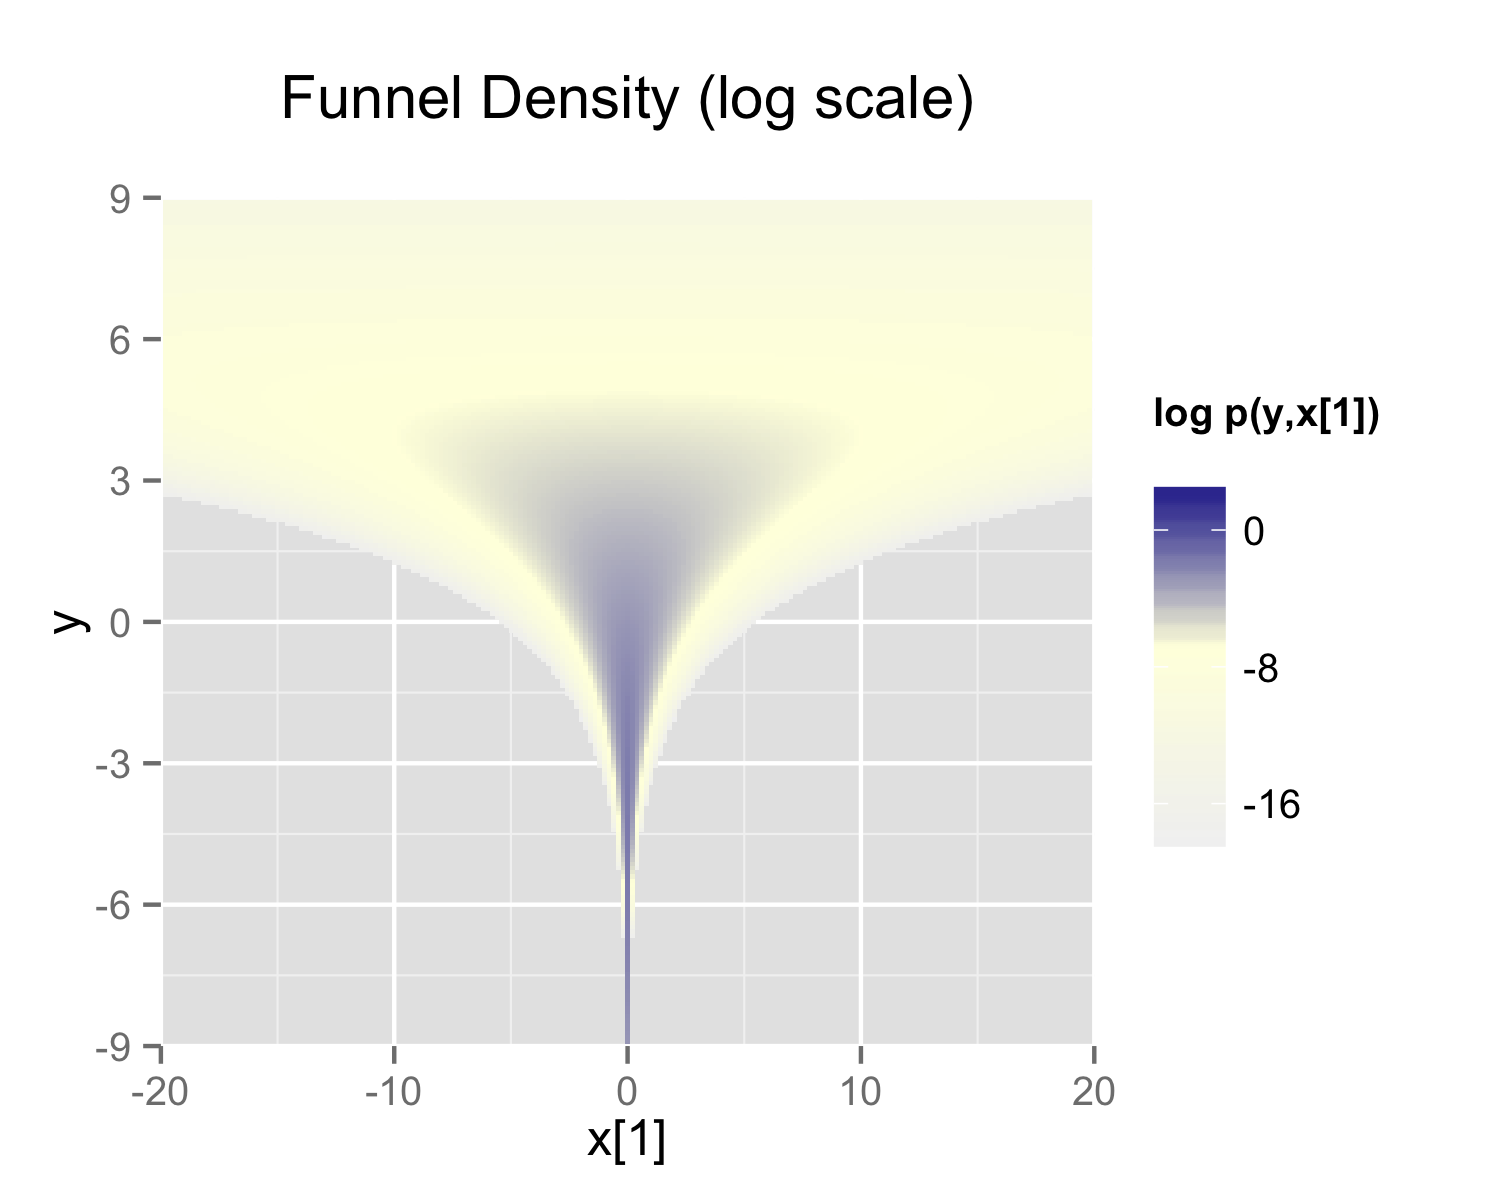
\includegraphics[height=2in]{R/funnel.png}
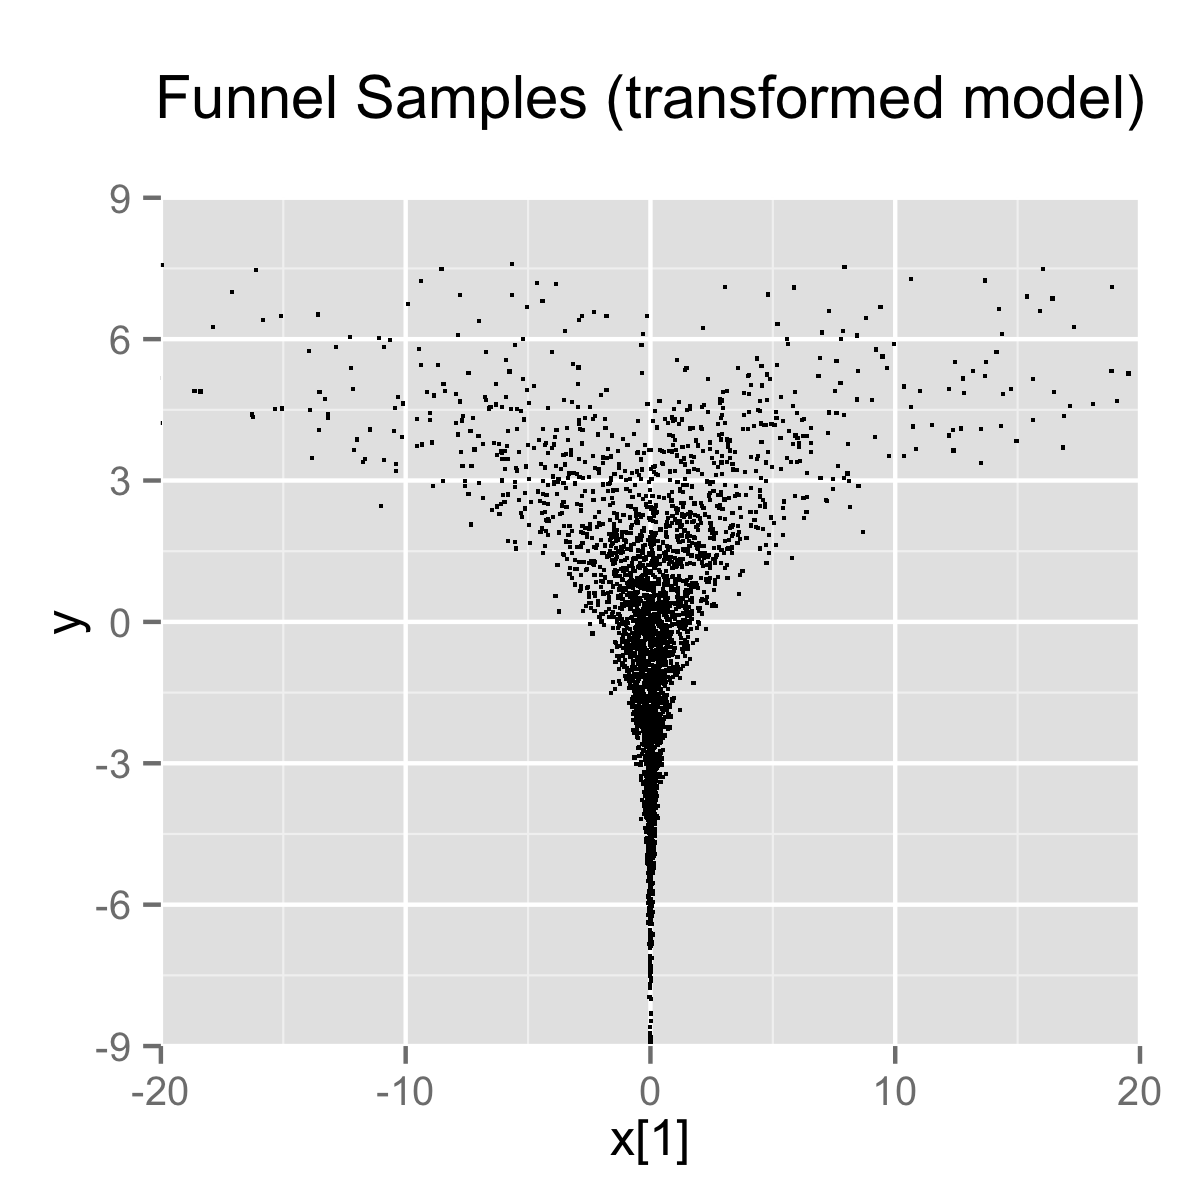
\includegraphics[height=2in]{R/funnel-fit.png}
\end{center}
\vspace*{-18pt}
\caption{\small \it Neal's Funnel.  (Left) The marginal density of
  Neal's funnel for the upper-level variable $y$ and one lower-level
  variable $x_1$ (see the text for the formula).  The blue region has
  log density greater than -4, the yellow region density less than
  -16, and the gray background a density less than -16.  The marginal
  standard deviation 3.  (Right) 4000 draws from a run of Stan's
  sampler with default settings.  Both plots are restricted to the
  shown window of $x_1$ and $y$ values; samples were drawn outside of
  this area as would be expected given the density.  The samples are
  consistent witht the marginal density $p(y) =
  \distro{Normal}(y|0,3)$, which has mean 0 and standard deviation
  3.}\label{funnel.figure}
\end{figure}

\citep{Neal:2003} defines a distribution that exemplifies the
difficulties of sampling from some hierarchical models.  Neal's
example is fairly extreme, but can be trivially reparameterized in
such a way as to make sampling straightforward.

Neal's example has support for $y \in
\mathbb{R}$ and  $x \in \mathbb{R}^9$ with density
%
\[
p(y,x) = \distro{Normal}(y|0,3) \times \prod_{n=1}^9
\distro{Normal}(x_n|0,\exp(y/2)).
\]
%
The probability contours are shaped like ten-dimensional funnels.  The
funnel's neck is particularly sharp because of the exponential
function applied to $y$.  A plot of the log marginal density of $y$
and the first dimension $x_1$ is shown in \reffigure{funnel}.

The funnel can be implemented directly in Stan as follows.
%
\begin{quote}
\begin{Verbatim}
parameters {  
  real y;
  vector[9] x;
}
model {
  y ~ normal(0,3);
  x ~ normal(0,exp(y/2));
}
\end{Verbatim}
\end{quote}
%
When the model is expressed this way, Stan has trouble sampling from
the neck of the funnel, where $y$ is small and thus $x$ is constrained
to be near 0.  This is due to the fact that the density's scale
changes with $y$, so that a step size that works well in the body will
be too large for the neck and a step size that works in the neck will be
very inefficient in the body.

In this particular instance, because the analytic form of the density
from which samples are drawn is known, the model can be converted to
the following more efficient form.
%
\begin{quote}
\begin{Verbatim}
parameters {  
  real y_raw;
  vector[9] x_raw;
}
transformed parameters {
  real y;
  vector[9] x;

  y <- 3.0 * y_raw;       // implies y ~ normal(0,3)
  x <- exp(y/2) * x_raw;  // implies x ~ normal(0,exp(y/2))
}
model {
  y_raw ~ normal(0,1);  
  x_raw ~ normal(0,1);  
}
\end{Verbatim}
\end{quote}
%
In this second model, the parameters \Verb|x_raw| and \Verb|y_raw| are
sampled as independent unit normals, which is easy for Stan.  These
are then transformed into samples from the funnel.  In this case, the
same transform may be used to define Monte Carlo samples directly
based on independent unit normal samples; Markov chain Monte Carlo
methods are not necessary. If such a reparameterization were used in
Stan code, it is useful to provide a comment indicating what the
distribution for the parameter implies for the distribution of the
transformed parameter.

\subsection{Hierarchical Models}

Unfortunately, the usual situation in applied Bayesian modeling
involves complex geometries and interactions that are not known
analytically.  Nevertheless, reparameterization can still be very
effective for separating parameters.  For example, a vectorized
hierarchical model might draw a vector of coefficients $\beta$ with
definitions as follows.
%
\begin{quote}
\begin{Verbatim}
parameters {
  real mu_beta;   
  real<lower=0> sigma_beta;
  vector[K] beta;
  ...
model {
  beta ~ normal(mu_beta,sigma_beta);
  ...
\end{Verbatim}
\end{quote}
%
Although not shown, a full model will have priors on both
\Verb|mu_beta| and \Verb|sigma_beta| along with data modeled based on
these coefficients.  For instance, a standard binary logistic
regression with data matrix \code{x} and binary outcome vector
\code{y} would include a likelihood statement such as form
\Verb|y ~ bernoulli_logit(x * beta)|, leading to an analytically
intractable posterior.

A hierarchical model such as the above will suffer from the same kind
of inefficiencies as Neal's funnel, though typically not so extreme,
because the values of \Verb|beta|, \Verb|mu_beta| and
\Verb|sigma_beta| are highly correlated in the posterior.  Such a
hierarchical model can be made much more efficient in terms of
effective sample size by reparameterizing in exactly the same way as
the funnel example.
%
\begin{quote}
\begin{Verbatim}
parameters {
  vector[K] beta_raw;
  ...
transformed parameters {
  vector[K] beta;
  // implies: beta ~ normal(mu_beta,sigma_beta)
  beta <- mu_beta + sigma_beta * beta_raw;
model {
  beta_raw ~ normal(0,1);  
  ...
\end{Verbatim}
\end{quote}
%
Any priors defined for \Verb|mu_beta| and \Verb|sigma_beta| remain as
defined in the original model.

Reparameterization of hierarchical models is not limited to the normal
distribution, although the normal distribution is the best candidate
for doing so. In general, any distribution of parameters in the 
location-scale family is a good candidate for reparameterization. Let
$\beta = l + s\alpha$ where $l$ is a location parameter and $s$ is a
scale parameter. Note that $l$ need not be the mean, $s$ need not
be the standard deviation, and neither the mean nor the standard
deviation need to exist. If $\alpha$ and $\beta$ are from the same
distributional family but $\alpha$ has location zero and unit scale, 
while $\beta$ has location $l$ and scale $s$, then that distribution
is a location-scale distribution. Thus, if $\alpha$ were a parameter
and $\beta$ were a transformed parameter, then a prior distribution
from the location-scale family on $\alpha$ with location zero and unit 
scale implies a prior distribution on $\beta$ with location $l$ and
scale $s$. Doing so would reduce the dependence between $\alpha$, 
$l$, and $s$.

There are several univariate distributions in the location-scale
family, such as the Student t distribution, including its special
cases of the Cauchy distribution (with one degree of freedom) and the
normal distribution (with infinite degrees of freedom). As shown above,
if $\alpha$ is distributed standard normal, then $\beta$ is distributed
normal with mean $\mu = l$ and standard deviation $\sigma = s$. The 
logistic, the double exponential, the generalized extreme value 
distributions, and the stable distribution are also in the 
location-scale family.

\subsection{Multivariate Reparameterizations}

The benefits of reparameterization are not limited to univariate 
distributions. A parameter with a multivariate normal prior distribution
is also an excellent candidate for reparameterization. Suppose you intend
the prior for $\beta$ to be multivariate normal with mean vector $\mu$
and covariance matrix $\Sigma$. Such a belief is reflected by the
following code.
%
\begin{quote}
\begin{Verbatim}
data {
  int<lower=2> K;
  vector[K] mu;
  cov_matrix[K] Sigma;
  ...
parameters {
  vector[K] beta;
  ...
model {
  beta ~ multi_normal(mu,Sigma);
  ...
\end{Verbatim}
\end{quote}
%
In this case \Verb|mu| and \Verb|Sigma| are fixed data, but they could
be unknown parameters, in which case their priors would be unaffected
by a reparameterization of \Verb|beta|.

If $\alpha$ has the same dimensions as $\beta$ but the elements of 
$\alpha$ are independently and identically distributed standard normal 
such that $\beta = \mu + L\alpha$, where $LL^\top = \Sigma$, then 
$\beta$ is distributed multivariate normal with mean vector $\mu$ and 
covariance matrix $\Sigma$. One choice for $L$ is the Cholesky factor
of $\Sigma$. Thus, the model above could be reparameterized as follows.
%
\begin{quote}
\begin{Verbatim}
data {
  int<lower=2> K;
  vector[K] mu;
  cov_matrix[K] Sigma;
  ...
transformed data {
  matrix[K,K] L;
  L <- cholesky_decompose(Sigma);
}
parameters {
  vector[K] alpha;
  ...
transformed parameters {
  vector[K] beta;
  beta <- mu + L * alpha; 
}
model {
  alpha ~ normal(0,1); 
  // implies: beta ~ multi_normal(mu, Sigma)
  ...
\end{Verbatim}
\end{quote}
%
This reparameterization is more efficient for two reasons. First, it
reduces dependence among the elements of \Verb|alpha| and second, it
avoids the need to invert \Verb|Sigma| every time \Verb|multi_normal|
is evaluated.

The Cholesky factor is also useful when a covariance matrix is 
decomposed into a correlation matrix that is multiplied from both
sides by a diagonal matrix of standard deviations, where either the
standard deviations or the correlations are unknown parameters. The
Cholesky factor of the covariance matrix is equal to the product of
a diagonal matrix of standard deviations and the Cholesky factor of
the correlation matrix. Furthermore, the product of a diagonal matrix
of standard deviations and a vector is equal to the elementwise
product between the standard deviations and that vector. Thus, if for
example the correlation matrix \Verb|Tau| were fixed data but the
vector of standard deviations \Verb|sigma| were unknown parameters,
then a reparameterization of \Verb|beta| in terms of \Verb|alpha|
could be implemented as follows.
%
\begin{quote}
\begin{Verbatim}
data {
  int<lower=2> K;
  vector[K] mu;
  corr_matrix[K] Tau;
  ...
transformed data {
  matrix[K,K] L;
  L <- cholesky_decompose(Tau);
}
parameters {
  vector[K] alpha;
  vector<lower=0>[K] sigma;
  ...
transformed parameters {
  vector[K] beta;
  // This equals mu + diag_matrix(sigma) * L * alpha;
  beta <- mu + sigma .* (L * alpha);
}
model {
  sigma ~ cauchy(0,5);
  alpha ~ normal(0,1);
  // implies: beta ~ multi_normal(mu,
  //  diag_matrix(sigma) * L * L' * diag_matrix(sigma)))
  ...
\end{Verbatim}
\end{quote}
%
This reparameterization of a multivariate normal distribution in
terms of standard normal variates can be extended to other multivariate
distributions that can be conceptualized as contaminations of the 
multivariate normal, such as the multivariate Student t and the skew
multivariate normal distribution.

Another candidate for reparameterization is the Dirichlet distribution
with all $K$ shape parameters equal. \citep{ZyczkowskiSommers:2001} shows 
that if $\theta_i$ is equal to the sum of $\beta$ independent squared 
standard normal variates and $\rho_i = \frac{\theta_i}{\sum \theta_i}$, 
then the $K$-vector $\rho$ is distributed Dirichlet with all shape 
parameters equal to $\frac{\beta}{2}$. In particular, if $\beta = 2$, 
then $\rho$ is distributed uniformally on the unit simplex. Thus, we can 
make $\rho$ be a transformed parameter to reduce dependence, as in:
%
\begin{quote}
\begin{Verbatim}
data {
  int<lower=1> beta;
  ...
parameters {
  vector[K] z[beta];
  ...
transformed parameters {
  simplex[K] rho;
  for (k in 1:K)
    rho[k] <- dot_self(z[k]); // sum-of-squares
  rho <- rho / sum(rho);
}
model {
  z ~ normal(0,1); 
  // implies: rho ~ dirichlet(0.5 * beta * ones)
  ...
\end{Verbatim}
\end{quote}
%
\section{Vectorization}

\subsection{Gradient Bottleneck}

\Stan spends the vast majority of its time computing the gradient of
the log probability function, making gradients the obvious target for
optimization.  \Stan's gradient calculations with algorithmic
differentiation require a template expression to be allocated%
%
\footnote{\Stan uses its own arena-based allocation, so allocation and
  deallocation are faster than with a raw call to \code{new}.}
%
and constructed for each subexpression of a \Stan program involving
parameters or transformed parameters.  This section defines
optimization strategies based on vectorizing these subexpressions to
reduce the work done during algorithmic differentiation.

\subsection{Vectorizing Summations}

Because of the gradient bottleneck described in the previous section,
it is more efficient to collect a sequence of summands into a vector
or array and then apply the \code{sum()} operation than it is to
continually increment a variable by assignment and addition.  For
example, consider the following code snippet, where \code{foo()} is
some operation that depends on \code{n}.
%
\begin{quote}
\begin{Verbatim}
for (n in 1:N) 
   total <- total + foo(n,...);
\end{Verbatim}
\end{quote}
%
This code has to create intermediate representations for each
of the \code{N} summands.  

A faster alternative is to copy the values into a vector, then
apply the \code{sum()} operator, as in the following refactoring.
%
\begin{quote}
\begin{Verbatim}
{  
  vector[N] summands;
  for (n in 1:N) 
    summands[n] <- foo(n,...);
  total <- sum(summands);
}
\end{Verbatim}
\end{quote}
%
Syntactically, the replacement is a statement block delineated
by curly brackets (\Verb|{|, \Verb|}|), starting with the definition
of the local variable \code{summands}.

Even though it involves extra work to allocate the \code{summands}
vector and copy \code{N} values into it, the savings in
differentiation more than make up for it.  Perhaps surprisingly,
it will also use substantially less memory overall than incrementing
\code{total} within the loop.


\subsection{Vectorization through Matrix Operations}

The following program directly encodes a linear regression with fixed
unit noise using a two-dimensional array \code{x} of predictors, an
array \code{y} of outcomes, and an array \code{beta} of regression
coefficients.
%
\begin{quote}
\begin{Verbatim}
data {
    int<lower=1> K;
    int<lower=1> N;
    real x[K,N];
    real y[N];
}
parameters {
    real beta[K];
}
model {
    for (n in 1:N) {
        real gamma;  gamma <- 0.0;
        for (k in 1:K)
            gamma <- gamma + x[n,k] * beta[k];
        y[n] ~ normal(gamma,1);
    }
}
\end{Verbatim}
\end{quote}
%
The following model computes the same log probability function as the
previous model, even supporting the same input files for data and
initialization.
%
\begin{quote}
\begin{Verbatim} 
data {
    int<lower=1> K;
    int<lower=1> N;
    vector[K] x[N];
    real y[N];
}
parameters {
    vector[K] beta;
}
model {
    for (n in 1:N)
        y[n] ~ normal(dot_product(x[n],beta), 1);
}
\end{Verbatim}
\end{quote}
%
Although it produces equivalent results, the dot product should not be
replaced with a transpose and multiply, as in
%
\begin{quote}
\begin{Verbatim} 
        y[n] ~ normal(x[n]' * beta, 1);
\end{Verbatim}
\end{quote}
%
The relative inefficiency of the transpose and multiply approach is
that the transposition operator allocates a new vector into which the
result of the transposition is copied.  This consumes both time
and memory.
%
\footnote{Future versions of \Stan may remove this inefficiency
by more fully exploiting expression templates inside the Eigen
\Cpp matrix library.  This will require enhancing Eigen to deal
with mixed-type arguments, such as the type \code{double} used
for constants and the algorithmic differentiation type
\code{stan::agrad::var} 
used for variables.}
%
The inefficiency of transposition could itself be mitigated somewhat by
reordering the product and pulling the transposition out of the loop,
as follows.
%
\begin{quote}
\begin{Verbatim} 
...
transformed parameters {
    row_vector[K] beta_t;
    beta_t <- beta';
}
model {
    for (n in 1:N)
        y[n] ~ normal(beta_t * x[n], 1);
}
\end{Verbatim}
\end{quote}
%
The problem with transposition could be completely solved by directly
encoding the \code{x} as a row vector, as in the
following example.
%
\begin{quote}
\begin{Verbatim} 
data {
    ...
    row_vector[K] x[N];
    ...
}
parameters {
    vector[K] beta;
}
model {
    for (n in 1:N)
        y[n] ~ normal(x[n] * beta, 1);
}
\end{Verbatim}
\end{quote}
%
Declaring the data as a matrix and then computing all the predictors
at once using matrix multiplication is more efficient still, as in the
example discussed in the next section.

\subsection{Vectorized Probability Functions}

The final and most efficient version replaces the loops and
transformed parameters by using the vectorized form of the normal
probability function, as in the following example.
%
\begin{quote}
\begin{Verbatim} 
data {
    int<lower=1> K;
    int<lower=1> N;
    matrix[N,K] x;
    vector[N] y;
}
parameters {
    vector[K] beta;
} 
model {
    y ~ normal(x * beta, 1);
}
\end{Verbatim}
\end{quote}
%
The variables are all declared as either matrix or vector types.
The result of the matrix-vector multiplication \code{x * beta} in the
model block is a vector of the same length as \code{y}.  

The probability function documentation in \refpart{built-in-functions}
indicates which of \Stan's probability functions support
vectorization; see \refsection{prob-vectorization} for more
information.  Vectorized probability functions accept either vector or
scalar inputs for all arguments, with the only restriction being that
all vector arguments are the same dimensionality.  In the example
above, \code{y} is a vector of size \code{N}, \code{x * beta} is a
vector of size \code{N}, and \code{1} is a scalar.

\section{Exploiting Sufficient Statistics}

In some cases, models can be recoded to exploit sufficient statistics
in estimation.  This can lead to large efficiency gains compared to an
expanded model.  For example, consider the following Bernoulli
sampling model.
%
\begin{quote}
\begin{Verbatim}
data {
    int<lower=0> N;
    int<lower=0,upper=1> y[N];
    real<lower=0> alpha;
    real<lower=0> beta;
}
parameters {
    real<lower=0,upper=1> theta;
}
model {
    theta ~ beta(alpha,beta);
    for (n in 1:N) 
        y[n] ~ bernoulli(theta);
}
\end{Verbatim}
\end{quote}
%
In this model, the sum of positive outcomes in \code{y} is a
sufficient statistic for the chance of success \code{theta}.  The
model may be recoded using the binomial distribution as follows.
%
\begin{quote}
\begin{Verbatim}
    theta ~ beta(alpha,beta);
    sum(y) ~ binomial(N,theta);
\end{Verbatim}
\end{quote}
%
Because truth is represented as one and falsehood as zero, the sum
\code{sum(y)} of a binary vector \code{y} is equal to the number of
positive outcomes out of a total of \code{N} trials.  



\section{Exploiting Conjugacy}


Continuing the model from the previous section, the conjugacy of the
beta prior and binomial sampling distribution allow the model to be
further optimized to the following equivalent form.
%
\begin{quote}
\begin{Verbatim}
    theta ~ beta(alpha + sum(y), beta + N - sum(y));
\end{Verbatim}
\end{quote}
%
To make the model even more efficient, a transformed data variable
defined to be \code{sum(y)} could be used in the place of \code{sum(y)}.


% \section{Using Forward Sampling}

% In fact, at this point, simple (non Markov chain) Monte Carlo may be
% used because the parameters to the beta distribution are specified and
% there are no variables that depend on \code{theta}.  Thus this model
% could be even further optimized by replacing the declaration of
% \code{theta} as a parameter with a declaration as a generated quantity
% and then generating the quantity directly.
% %
% \begin{quote}
% \begin{Verbatim}
% generated quantities {
%     real<lower=0,upper=1> theta;
%     theta ~ random_beta(alpha + sum(y), beta + N - sum(y));
% }
% \end{Verbatim}
% \end{quote}
% %
% When used in the generated quantities block, sampling statements such
% as that for \code{theta} are executed by taking a sample from the
% specified distribution directly. The result is a Monte Carlo estimate
% of \code{theta} in which every sample is independent (up to the limits
% of the pseudorandom number generator, of course).  Thus the effective
% sample size should be estimated as being roughly equal to the sample
% size.
